 \documentclass[book.tex]{subfiles}
\begin{document}

\section{Tricks}

This section describes random tricks used to speed up rendering. 




\subsection{Bouncing Flower}
When Keen throws a flower it bounces of the walls. For flat walls and floors the bounce can be easily calculated by reversing either the x-speed (for vertical walls) or y-speed (for horizontal walls). It becomes more complicated for slopes. Making an accurate calculation of the bounce on a slope requires expensive \cw{cos} and \cw{sin} methods. \\
\par
Instead, the game used a simple algorithm that approximates the angle to either 22$^{\circ}$, 45$^{\circ}$ or 90$^{\circ}$. Based on the ratio between the x- and y-speed it calculates the resulting speed and corresponding angle. Notice that for higher precision the speed is multiplied with 256.\\
\par
\begin{figure}[H]
\centering
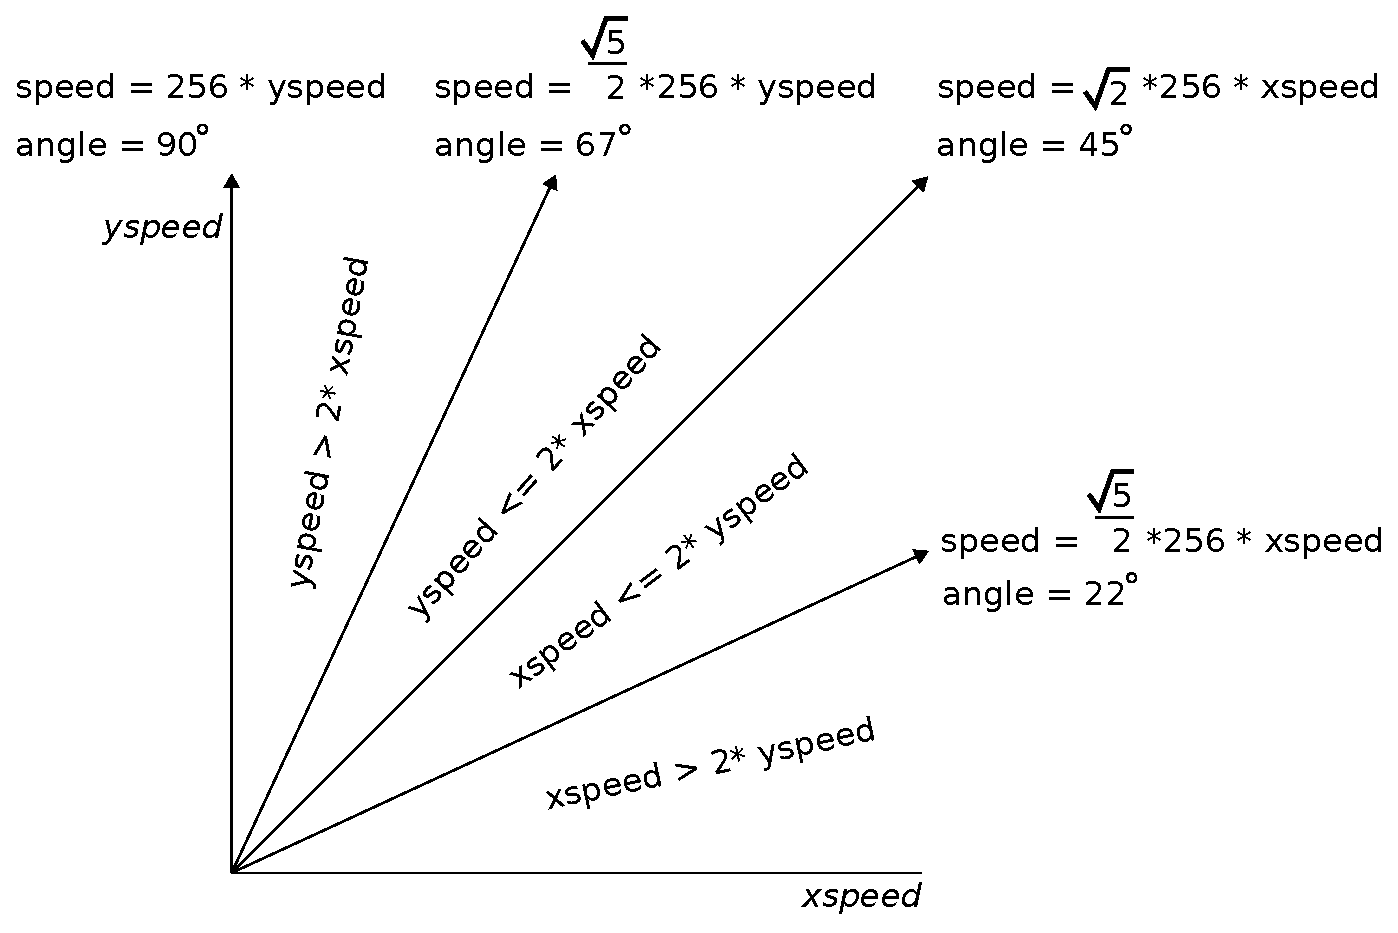
\includegraphics[width=0.8\textwidth]{imgs/drawings/angle.eps}
\label{fig:angles}
\end{figure}
\par

For each of the eight type of slopes (Figure \ref{fig:walltype}) and incoming angle combination, the corresponding bounce is defined using a simple lookup table.\\

\par
\begin{minipage}{\textwidth}
  \lstinputlisting[language=C]{code/bounceangle_lookup.c}
\end{minipage}
\label{wallclip_array}
\par

The value in the table refers to the corresponding bounce angle calculation.

\par
\begin{figure}[H]
\centering

\includegraphics[width=0.7\textwidth]{imgs/drawings/bounce_angle.eps}
\caption{Walltype 3 with incoming angle of 22$^{\circ}$ (angle=0).}
\label{fig:bounce_angles}
\end{figure}
\par

\par
\begin{minipage}{\textwidth}
  \lstinputlisting[language=C]{code/angle.c}
\end{minipage}
\label{wallclip_array}
\par

Notice that in several cases the bounce angle is not following the laws of physics.
\par
\begin{figure}[H]
\centering

\includegraphics[width=0.4\textwidth]{imgs/drawings/bounce_physics.eps}
\caption{Incoming angle of 22$^{\circ}$ on a 45$^{\circ}$ slope results in 90$^{\circ}$ bounce.}
\label{fig:bounce_angles}
\end{figure}
\par



\section{Pseudo Random Generator}
Random numbers are necessary for many things during runtime, such as calculating whether an enemy is able to hit the player based on its accuracy. This is achieved with a precalculated pseudo-random series of 256 elements.\\
\par
\begin{minipage}{\textwidth}
\lstinputlisting[language={[x86masm]Assembler}, style=mystyle,basicstyle=\small]{code/rndtable.asm}
\end{minipage}
\par
 Each entry in the array has a dual function. It is an integer within the range [0-255]\footnote{Or at least it was intended to!} and it is also the index of the next entry to fetch for next call. This works overall as a 255 entry chained list. The pseudo-random series is initialized using the current time modulo 256 when the engine starts up.\\

\par
\begin{minipage}{\textwidth}
\lstinputlisting[language={[x86masm]Assembler}]{code/US_InitRndT.asm}
\end{minipage}\\
\par
The random number generator saves the last index in \cw{rndindex}. Upon request for a new number, it simply looks up the new value and updates \cw{rndindex}.
\par
\begin{minipage}{\textwidth}
\lstinputlisting[ language={[x86masm]Assembler}]{code/US_RndT.asm}
\end{minipage}



\end{document}



